%#!platex -kanji=utf8 hb.tex
\chapter{書式・ページ設定}\chaplab{書式・ページ設定}
% これはただのダミーテキスト.
% 文字コードを判定するための意味のない文字列.
% これくらい記述すれば大丈夫かな.
% Emacs のくせに生意気な.
% Emacs の分際で自動判別とか.
% Mac OS X のテキストエディッタの文字コード自動判別はうまくいかないぞ.



% 文書の書式・体裁を決定する 
\section{書式}

\section{クラスとパッケージ}\seclab{class}
{\LaTeX}は\Z{マークアップ}方式を採用した言語なので\Z{書式}と内容は
分離されるのが一般的です.そこで\Z{クラス}\pp{\Z{class}}と
\Z{パッケージ}\pp{\Z{package}}という二つのファイルを使う
ようになっています.

%さて,クラスやパッケージという用語が出てきましたが,簡単
%に説明しましょう.昔の話は置いといて\pp{{\LaTeX2.09}},
{\LaTeX}では文書の書式を決定するためにクラスというもの
を宣言します.クラスは\Z{ドキュメントクラス}とか
\Z{文書クラス}などと呼ばれています.また,便利な機能%
\zindind{マクロ}{パッケージ}%
を集めたものを\K{パッケージ}と呼びます.パッケージは\K{マクロパッケージ}
とか,ただ単に\KY{マクロ}などと呼ばれます.

そうして,{\LaTeX}の原稿\pp{\Z{ソースファイル}}では必ず文
書の先頭にHOGE
のような記述をして,文書の書式を大雑把に決定します.
\begin{usage}
\documentclass[$\<オプション>,\ldots$]{$\<クラス>$}
\end{usage}
%\begin{Syntax}
%\cmd{documentclass}\opa{オプション$,\ldots$}\pa{クラス}\\ 
%\cmd{usepackage}\opa{オプション$,\ldots$}\pa{パッケージ}
%%\cmd{documentclass}\opa{オプション}\pa{クラス}\\ 
%%\cmd{usepackage}\opa{オプション}\pa{パッケージ}
%\end{Syntax}


%例えば,日本語の小規模の画像を含み,書体の大きさが11ポイントで
%\Z{2段組}の記事を書こうと思えば
例えば,本文が日本語で画像を含み,書体の大きさが11ポイントで
\Z{2段組}の記事を書こうと思えば次のように原稿中で宣言します.

\begin{intext}
\documentclass[twocolumn,11pt]{jarticle}
\usepackage[dvips]{color}
\usepackage[dvips]{graphicx}
\end{intext}

使用するクラスの中にはオプションが
存在し,上記のように2段組のために\option{twocolumn}やフォントの
大きさを指定するために\option{11pt}というオプションを指定します.
また衝突の起きない限り,複数のパッケージを使う事を
同時に宣言する事もできます.

\begin{intext}
\documentclass[twocolumn,11pt]{jarticle}
\usepackage[dvips]{graphicx,color}
\end{intext}

クラスとパッケージを明確に区別するために
クラスの\Z{拡張子}には\exten{cls}を,
パッケージの拡張子には\exten{sty}を付けるようにします.

\subsection{標準的なクラス}\seclab{01pregame:sec:classes}

\indindz{クラス}{標準的な}%
{\LaTeX}や{\pLaTeX}の範囲内で提供されている標準的なクラスを
紹介します.クラスファイルは\Va{classes}{dtx}と
\Va{classes}{ins}という二つのファイルで配布される事が多い
ようです.

あるクラスが何からインストールできるのかは,すでにでき
上がっているクラスファイル\Va{classes}{cls}が存在すれば
そのファイルの先頭部分に次のような記述があります.

\begin{intext}
%% This is file `class.cls',
%% generated with the docstrip utility.
%% The original source files were:
%% classes.dtx  (with options: `option')
\end{intext}

オリジナルのソースファイルは
オプションに\option{`option'}を指定してファイル名が
\Va{classes}{dtx}です,と説明してくれていますので
Unix系OSならば
%\begin{InTerm}
%  \type{find /usr/local/share/texmf/ -name classes.dtx}
%\end{InTerm}
などでそのファイルを検索できるでしょう.WindowsやMacintosh
はファイルの検索の機能があると思いますので,そちらを使えば
良いでしょう.そのようにして検索した場所に\Va{classes}{dtx}や
\Va{classes}{ins}が存在します.そのファイルがある場所に移動して
%\begin{InTerm}
  \type{platex classes.dtx}
%\end{InTerm}
とすればそのクラスの仕様書を見る事ができます.さらに
%\begin{InTerm}
  \type{platex classes.ins}
%\end{InTerm}
とするとそのクラスを導入する事ができます.このような操作をすると
\Sty{DocStrip}というマクロが適切にファイルを処理します.
例えばファイル\Fl{classes.ins}をこのように処理すると,
\Fl{article.cls},\Fl{report.cls},\Fl{book.cls},\Fl{bk10.clo},
\Fl{bk11.clo},\Fl{bk12.clo},\Fl{size10.clo},\Fl{size11.clo},
\Fl{size12.clo}という九つのファイルが生成されます.

日本語を含まないような文書には欧文専用のクラスが使用できます.
それぞれどのような文書を作成したいかによって何を用いるかが
分かれます.標準では以下の欧文用のクラスが使えます.
\begin{namelist}{xxxx}
\item[\Cls{article}] 小規模の記事を作成するためのクラス.
%	\Fl{classes.dtx}や{\COMP}に詳しい仕様が書かれている.
\item[\Cls{report}]  報告書を作成するためのクラス.
%	同じく\Fl{classes.dtx}や{\COMP}に詳しい仕様が書かれている.
\item[\Cls{book}]    書籍を作成するためのクラス.
%	同じく\Fl{classes.dtx}や{\COMP}に詳しい仕様が書かれている.
\item[\Cls{slides}]  スライドを作成するためのクラス.
%	\Fl{slides.dtx}に詳しい仕様が書かれている.
\item[\Cls{proc}]    \cls{article}をベースに議事録などを%
	作成するためのクラス.
%	\Fl{proc.dtx}に詳しい仕様が書かれている.
\end{namelist}
以上の\cls{article},\cls{report},\cls{book}の三つをまとめて
\Cls{classes}と呼ぶ事があります.

日本語の文書では,標準で以下のクラスが使えます.
\begin{namelist}{xxxxx}
\indindz{クラス}{小規模な文書用の}
\item[\Cls{jarticle}] 小規模の日本語の記事を作成するためのクラス.
\indindz{クラス}{報告書用の}
\item[\Cls{jreport}]  日本語の報告書を作成するためのクラス.
\indindz{クラス}{書籍用の}
\item[\Cls{jbook}]    日本語の書籍を作成するためのクラス.
\item[\Cls{tarticle}] 縦書きの小規模の日本語の記事を作成するためのクラス.
\item[\Cls{treport}]  縦書きの日本語の報告書を作成するためのクラス.
\item[\Cls{tbook}]    縦書きの日本語の書籍を作成するためのクラス.
\end{namelist}
以上の\cls{jarticle},\cls{jreport},\cls{jbook}の三つをまとめて
\Cls{jclasses}と呼ぶ事があります.

\subsection{クラスオプション}\seclab{classopt}
ドキュメントクラス\pp{文書クラス}にはもう少し詳細な
設定を行う事ができます.\cmd{documentclass}の任意引数として
記述します.多くのクラスファイルでは次の\Z{クラスオプション}が
使えると思います.
\begin{description}
\item[{文字サイズ}{\Optionlist{10pt,11pt,12pt}}] 
\zindind{文字}{サイズ}%
\zindind{原稿}{の文字サイズ}%
原稿で基本となる文字の大きさを決めます.この文字サイズを
基準としてさまざまなパラメータが設定されます.標準は
\option{10pt}.

\item[{用紙サイズ}{\Optionlist{a4paper,a5paper,b5paper,letterpaper}}]
原稿の用紙の大きさを指定します.
\index{用紙!\zdash のサイズ}%
\index{用紙!\zdash の大きさ}%
\zindind{原稿}{の用紙サイズ}%
和文の場合はこの他に\Optionlist{b4paper,a4j,a5j,b4j,b5j}などです.
\sty{geometry}パッケージや\cls{jsclasses}を使うと選択の幅が
広がります.

\item[{用紙方向}{\Option{landscape}}]
用紙を横置きにします.標準は縦置きです.\index{用紙!\zdash の方向}

\item[\Z{印刷面}{\Optionlist{oneside,twoside}}]
用紙の片面\pp{\option{oneside}}だけに印刷するか
それとも両面\pp{\option{twoside}}に印刷するかを指定します.
\item[\Z{段組}{\Optionlist{onecolumn,twocolumn}}]
\indindz{段組}{1}\indindz{段組}{2}%
\Z{1段組}\pp{\option{onecolumn}}にするか\Z{2段組}\pp{\option{twocolumn}}
にするかを指定します.

\indindz{表題}{独立ページの}\indindz{表題}{同ページの}\indindz{ページ}{表題}
\item[{表題}{\Optionlist{titlepage,notitlepage}}]
表題を独立して出力する\pp{\option{titlepage}}か,
同じページに出力する\pp{\option{notitlepage}}かという表題の
レイアウトを指定します.

\item[{数式の位置}{\Option{fleqn}}]
\zindind{数式}{の位置}%	   
別行数式の位置を左揃えに指定します.標準は中央揃えです.
	
\item[{数式番号の位置}{\Option{leqno}}]
\zindind{数式}{番号の位置}%
数式番号の位置を左側に指定します.標準は右側です.
	
\item[\Z{ドラフト}{\Optionlist{draft,final}}]
\indindz{原稿}{ドラフト段階の}%
\indindz{原稿}{執筆段階の}%
執筆途中で印刷するときに\option{draft}オプションを付けると,
文書幅の領域をはみ出してしまった箇所に印が付いてくれます.
原稿が完成したら\option{final}に変更します.標準は\option{final}です.

\item[\Z{左右起し}{\Optionlist{openright,openany}}]
\cls{(j)report}や\cls{(j)book}において章などの開始ページの
指定をします.常に奇数ページで起こす\pp{\option{openright}}か,
どちらからでも起こす\pp{\option{openany}}かを設定します.
\cls{(j)report}の標準は\option{openany}.
\cls{(j)book}の標準は\option{openright}.
\end{description}


最近では,\Hito{奥村}{晴彦}が管理している
\Cls{jsclasses}というクラスファイル群に定評があります\footnote{\webJsclasses}.
このクラス群を導入すると
\begin{namelist}{xxxxxx}
\item[\Cls{jsarticle}]	小規模の日本語の記事を作成するためのクラス.
\item[\Cls{jsbook}]	日本語の書籍や報告書を作成するためのクラス.
\item[\Cls{jspf}]	某学会誌用のクラス.
\end{namelist}
の三つが使用できます.これらのクラスで指定できる
クラスオプションが\cls{jclasses}に追加されて
います\footnote{\cls{(j)classes}で定義されていたいくつかの
クラスオプションが実装されていません.}.
以上の\cls{jsarticle},\cls{jsbook},\cls{jspf}の三つをまとめて
\Cls{jsclasses}と呼びます.

\begin{description}
\item[\Z{文字サイズ}]{\Optionlist%
   {9pt,10pt,11pt,12pt,14pt,17pt,20pt,21pt,25pt,30pt,36pt,43pt,12Q,14Q}}
\item[\Z{用紙サイズ}]{\Optionlist%
   {a4paper,a5paper,a6paper,b5paper,b4paper,a4j,a5j,b4j,b5j,a4var,b5var}}
\item[言語の指定]{\Option{english}}
  欧文用の見出しの定義と行送りになります.
\item[用紙サイズ情報] {\Option{papersize}} 
  用紙サイズの情報をデバイスドライバに渡すようにします.
\item[レポート作成] {\Option{report}} 
  \Z{レポート作成}用に \cmd{chapter} 命令を使う事ができます.
  \cls{jsbook} では左右起し等に関する設定が変わります.
\end{description}





\subsection{大元の書式を指定する}
\begin{usage}
\documentclass[$\<オプション>$]{$\<クラスファイル>$} 
\end{usage}

\val{クラスファイル}

\C{documentclass} 命令は一つの文書に一度だけ,ファイルの先頭に記述します.


\begin{description}
 \item[article] 
 \item[report]
 \item[book]
 \item[slides]
\end{description}

\begin{description}
 \item[jarticle] 
 \item[jreport]
 \item[jbook]
\end{description}

\begin{description}
 \item[jsarticle] 
 \item[jsbook]
\end{description}

jsreport はありませんが,次のように\Option{report}を付ければ片面印刷用に
書式が設定されます.
\begin{intext}
\documentclass[report]{jsbook}
\end{intext}


\subsection{用紙サイズを設定する}
\begin{usage}
\documentclass[$\<用紙サイズオプション>$]{$\<クラスファイル>$} 
\end{usage}

\subsection{デバイスドライバに用紙サイズを渡す}

\begin{usage}
\AtBeginDvi{\special{papersize=$\<用紙の幅>$,$\<用紙の高さ>$}}
\end{usage}

\CI{AtBeginDvi}%
\CI{special}%
例えばJISのB5 (182\,mm $\times$ 257\,mm) であれば次のようにします.
\begin{intext}
\AtBeginDvi{\special{papersize=182mm,257mm}}
\end{intext}
原稿の先頭で次のような1行を追加するだけです.

\zindind{ドキュメントクラス}{オプション}%
\indindz{オプション}{ドキュメントクラス}%
\Y{jsclasses}ではドキュメントクラスオプションに \Option{papersize}
を指定するだけで同様の効果を得る事ができます.

\begin{intext}
\documentclass[papersize]{jsarticle}
\end{intext}

ただし,後述する\Y{geometry}パッケージと競合する事になります.


\subsection{用紙の方向を設定する}

\subsection{両面・片面印刷を設定する}

\subsection{別行数式の位置を左揃えにする}

\subsection{別行数式の番号を左に設定する}

\subsection{左右起しにする}

\subsection{段組みを指定する}

\section{ページの設定}

\section{長さの単位}\index{単位}
\subsection{\LaTeX での単位の取り決め}
\latexno{における単位}
\index{数値の代入}%

\index{=@\str{=}!代入としての\zdash}%
\index{=@\str{=}}%
先ほどは何らかの\Z{変数}(\Z{パラメータ})に数値を代入する時に
`\verb|\parindent=0pt |'
という記述がありました.これにはポイント
\qu{pt}という単位が使われています.
{\LaTeX}において使用できる\zindind{長さ}{の単位}長さの単位
\pp{\tabref{latexunit1}}は色々あります.ポイントは%
\indindz{長さ}{絶対的な}%
\Z{絶対的な長さ}ではないのでクラスファイルによって変わった
りプログラムによっても若干の違いがあります.
\begin{table}[htbp]
\begin{center}
\indindz{幅}{Mの字の}%
\indindz{高さ}{xの字の}%
\zindind{日本語}{の幅}%
\caption{{\LaTeX}で使用できる主な単位}\label{tab:latexunit1}
\begin{tabular}{c*3l}
\TR
\Th{単位}& \Th{読み}&  \Th{補足\pp{数値は概算}} & \Th{実際の長さ}\\
\MR
in& \Z{インチ}  &1\,in $=$ 25.4\,mm $=$ 72.27\,pt & \demowidth{1truein}\\
cm& \Z{センチメートル} &1\,cm $=$ 10\,mm $=$ 28.3\,pt    & \demowidth{1truecm}\\
mm& \Z{ミリメートル}   &1\,mm $=$ 2.83\,pt           & \demowidth{1truemm}\\
pt& \Z{ポイント}      &1\,pt $=$ 0.35\,mm           & \demowidth{1truept}\\
em& Mの字の幅と同じ. &使用中のフォントに依存    & \demowidth{1em}\\
ex& xの字の高さと同じ.&使用中のフォントに依存  & \demowidth{1ex}\\
zw& 日本語の一文字の幅.&使用中のフォントに依存   & \demowidth{1zw}\\
\BR
\end{tabular}
\end{center}
\end{table}
\hito{奥村}{晴彦}の\cls{jsclasses}ではクラスオプションに
\Option{10pt}以外のフォントサイズ指定がされている場合は%
\zindind{紙面}{の拡大縮小}%
\zindind{単位}{のずれ}%
紙面の拡大縮小を使っていますので単位がずれます.これには
各単位に\qu{\str{true}}を付けて長さを指定します.例えば
\qu{\str{cm}}ならば\qu{\str{truecm}}のようにします.
%このようにすると \Cmd{magstep}の影響がありません.
%↑はいらないよなぁ.


\subsection{ページ設定のパラメータを知る}
1段組みの場合のページ設定に関わるパラメータを
\figref{1段組のページ設定のパラメータ一覧}に示します.
\begin{figure}[htbp]
 \begin{center}
  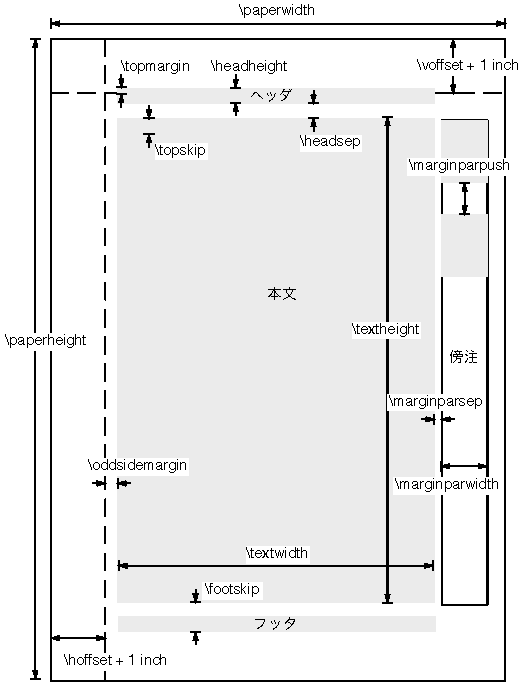
\includegraphics{layout}
  \caption{1段組のページ設定のパラメータ一覧}%
  \figlab{1段組のページ設定のパラメータ一覧}%
 \end{center}
\end{figure}

\index{用紙}
\zindind{ページ}{の余白}
次はページ全体の\W{余白}に関する長さです.
\begin{description}
 \item[\C{voffset}] \zindind{用紙}{の空白}
 横組みにおいて用紙の左上の部分に入れる縦方向の余白.
 この値を0にしてもすでに1インチ分の余白が\LaTeX 側で自動的に挿入されてい
  ます.
 本当に用紙の左上端から使うならば \cmd{voffset}を `\str{-1in}'に設定します.

 \item[\C{hoffset}] 
 横組みにおいて用紙の左上の部分に入れる横方向の余白.
 縦方向と同じようにすでに1インチ分の余白が挿入されています.

 \item[\C{oddsidemargin}]
ページが奇数のときに挿入される左側の余白.
文書クラスオプションに\Option{oneside}を
使っていると全てのページに \cmd{oddsidemargin}が
挿入されます.

 \item[\C{evensidemargin}] 
ページが偶数のときに挿入される左側の余白.
文書クラスオプションに\Option{twoside}を
使っているときだけ有効で\Option{oneside}では
意味がありません.
\end{description}

ヘッダの設定に関する長さです.
\begin{description}
\item[\C{topmargin}] 
\cmd{voffset}とヘッダの間隔です.
\item[\C{headheight}]
ヘッダの高さです.\indindz{高さ}{ヘッダの}%
\item[\C{headsep}]
ヘッダと本文領域の間隔です.
\item[\C{footskip}]
フッタ下部と本文領域の最下部との間隔です.
\end{description}

本文領域や傍注領域に関わる長さです.
\begin{description}
\item[\C{textheight}]\indindz{高さ}{本文領域の}%
 本文領域の高さです.ヘッダやフッタの高さは含まれません.
 \item[\C{textwidth}]
 本文領域の幅です.\indindz{幅}{本文の}%
 \item[\C{marginparwidth}]
  傍注の幅です.\indindz{幅}{傍注の}%
 \item[\C{marginparpush}]
 傍注と傍注のあいだの縦方向の長さです.
 \item[\C{marginparsep}]
 傍注と本文領域との間隔です.
\end{description}


\subsection{ページ設定のパラメータを個別に調整する}
\begin{usage}
\setlength{パラメータ}{設定値}
\end{usage}
\C{setlength}で \cmd{voffset}などの値を例えば 15\,mm に設定するには
次のようにします.
\begin{inonly}
\setlength{\voffset}{15mm}
\end{inonly}


\TeX/\LaTeX における\W{長さ}には伸縮するものと
しないもの2種類があります.伸縮するものを
{\W{可変長の長さ}}と呼び,伸縮しないものを\indindz{長さ}{可変長の}
{\W{固定長の長さ}}と呼びます.\indindz{長さ}{固定長の}
可変長の長さは{\W{スキップ}}と呼ばれる事が多いようですが,
本書では可変長の長さと呼びます.
可変長の長さは{\W{長さ}},
{\W{縮み率}},{\W{伸び率}}の三つの
属性を持っています.固定長の長さは決まった値しか
持ちません.可変長の長さは縮み率と伸び率に従って
バネのように伸縮します.長さの定義には \cmd{newlength}が使えます.
\begin{usage}
\newlength{$\<命令>$} 
\setlength{$\<命令>$}{$\<長さ>$}
\addtolength{$\<命令>$}{$\<長さ>$}
\end{usage}
%\begin{Syntax}
%\C{newlength}\pa{綴り}\\
%\C{setlength}\pa{綴り}\pa{長さ} \\
%\C{addtolength}\pa{綴り}\pa{長さ}
%\end{Syntax}
\cmd{setlength}で長さを設定します.\cmd{addtolength}
では元の長さにさらに長さを足します.\cmd{newlength}
で定義された長さは可変長にも固定長にもなって良い
事になっています.まず \cmd{newlength}で新規に
長さを定義します.次に \cmd{setlength}で
値を決めます.
\begin{inout}
\newlength{\newa}\the\newa\\
\setlength{\newa}{10mm}\the\newa\\
\setlength{\newa}{10mm plus 3mm
   minus 2mm}\the\newa\\
\addtolength{\newa}{3mm}\the\newa
\end{inout}
可変長の長さに値を足しても縮み率と伸び率には
影響しないのが例の出力から分かるでしょう.


\C{setlength}命令で個々のパラメータを調整する事も可能ですが,本書では
\Hito{梅木}{秀雄}の\Y{geometry}パッケージを用いたページ設定を中心に取り
上げます.\Y{geometry}を用いると%ユーザは細かい微調整を行わずに所望のレイ
%アウトを得る事が出来ます.
行数や余白を直感的に指定する事ができます.

\subsection{現在のページ設定を確認する}
\begin{usage}
\usepackage{layout}
\layout
\end{usage}
\Y{layout}パッケージを使うと,現在使用しているクラスファイルの
ページ設定を確認する事が出来ます.
\begin{inonly}
\documentclass[a5j,papersize]{jsarticle}
\usepackage{layout}
\begin{document}
\layout
\end{document}
\end{inonly}
\begin{outonly}
{\centering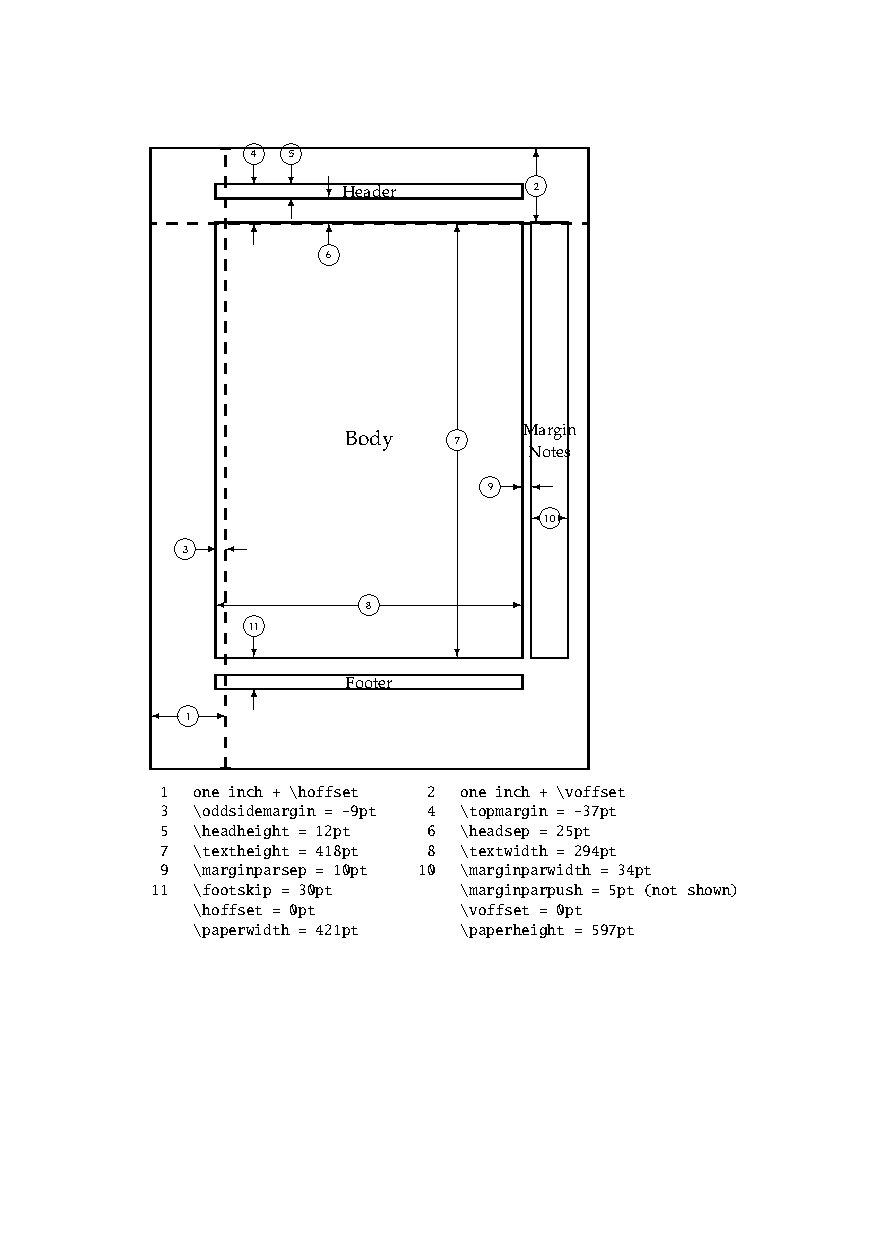
\includegraphics[width=.97\linewidth]{package-layout}}
\end{outonly}

\section{段組の変更}

\subsection{改ページを伴って1段組/2段組みを切り替える}
\CIS{onecolumn,twocolumn}
\begin{usage}
\onecolumn % 1 段組みに変更する
\twocolumn[$\<段落要素>$] % 2 段組みに変更する
\end{usage}
%\begin{Syntax}
%%\begin{tabular}{ll}
%% \C{onecolumn}           & \\
%% \C{twocolumn}\opa{要素} & \\
%%% \C{columnsep}          & \pp{2段組のときの段間}\\
%%% \C{columnseprule}      & \pp{2段組のときの段間に引く罫線の太さ}
%%\end{tabular}
%\end{Syntax}
1段組みにするためには \cmd{onecolumn}を使い,2段組に
するには \cmd{twocolumn}を使います.\cmd{twocolumn}
は改ページをしてから2段組を作成しようとします.
そのため任意引数に何らかの要素を与えるとその要素を
ページ上部に1段組で出力します.


\subsection{2段組のページレイアウト}

\CIS{columnseprule,columnsep}%
\begin{description}
  \item[\C{columnsep}]
 2段組以上での段と段の間隔です.
 \item[\C{columnseprule}]
 2段組以上での段と段のあいだに入る罫線です.\indindz{罫線}{2段組での}
\end{description}


\begin{figure}[htbp]
 \begin{center}
  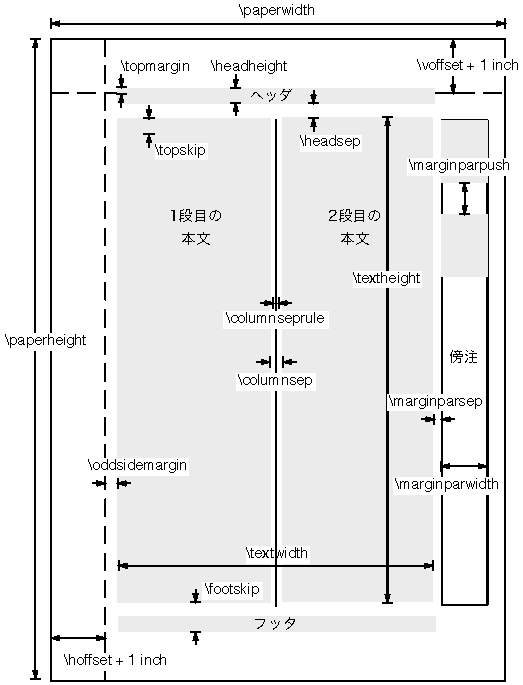
\includegraphics{layout-twocolumn}
  \caption{2段組のページ設定のパラメータ一覧}%
  \figlab{2段組のページ設定のパラメータ一覧}%
 \end{center}
\end{figure}

\subsection{最終ページの下端を揃える}
\Y{balance}パッケージ

\C{twocolumn}を使って2段組をすると最終ページの
段の高さが揃わないので,格好悪いでしょう.これは
\sty{multicol}パッケージで2段組にすると段が揃いますし,
\Sty{balance}パッケージを使っても可能です.

\subsection{3段組み以上}
\index{多段組}%
{\LaTeX}では通常1段組と2段組しか制御できません.
\zindind{2段組}{のときの段間}\zindind{2段組}{の段間の罫線}%


\Person{Frank}{Mittelbach}の作成した\Sty{multicol}を
使うと最高で10段まで段組できます.自動的に
段の終わりの最終ページの文章の高さを揃えてくれます.
星を付けると段の下端を揃えないようにするので,通常は星無しで用いると良い
でしょう.
\begin{usage}
\begin{multicols}{$\<段数>$}
$\<文章要素>$ 
\end{multicols} 
\end{usage}
%\begin{Syntax}
%\verb|\begin{multicols|\pa{段数}\\
%\val{文章内容}\\
%\verb|\end{multicols}| 
%\end{Syntax}
\Env{multicols}環境の場合は改ページされずに同じ
ページに違う段組を混在できます.余り好ましくない
事なので多用しないほうが良いでしょう.
以下のような入力があるとします.

\begin{inout}
\begin{multicols}{4}
このパッケージでは10段組まで多段組できますが, 同ページに違う段数の要素
を組み込むのは余り好ましいことではないので,特別な理由がない限り使うべき
ではありません.このパッケージでは段の終わりの最終ページの文章を自動で揃
えるので,従来の組版の規則にも合っています.
\end{multicols} 
\end{inout}

%そうすると,次のような出力を得ることができます.

%\begin{multicols}{4}
%このパッケージでは10段組まで多段組できますが, 
%同ページに違う段数の要素を組み込むのは余り
%好ましいことではないので,特別な理由がない限り
%使うべきではありません.このパッケージでは段の
%終わりの最終ページの文章を自動で揃えるので,従
%来の組版の規則にも合っています.
%\end{multicols} 

%\LaTeXe の標準では \C{onecolumn} と \C{twocolumn} によって 1 段組みと 2
%段組みを切替える事もできます.

%\begin{intext}
%\documentclass[twocolumn]{jsarticle}
%\end{intext}

%これによって全体の段組みを指定する事もできます.しかし, \C{onecolumn} と \C{twocolumn}
%の両方とも改ページが必須で,ページの途中で段を変更する事もできなければ,
%2 段組みのときに段の終わりが揃わないなどの制約があります .

\C*{multicolsep}%
\begin{intext}
\multicolsep=1zw % 段の上端/下端の空き
\end{intext}

\begin{inout}
\multicolsep=1zw % 段の上端/下端の空き
\begin{multicols}{4}
このパッケージでは10段組まで多段組できますが, 同ページに違う段数の要素
を組み込むのは余り好ましいことではないので,特別な理由がない限り使うべき
ではありません.このパッケージでは段の終わりの最終ページの文章を自動で揃
えるので,従来の組版の規則にも合っています.
\end{multicols} 
\multicolsep=2zw % 段の上端/下端の空き
\begin{multicols}{4}
このパッケージでは10段組まで多段組できますが, 同ページに違う段数の要素
を組み込むのは余り好ましいことではないので,特別な理由がない限り使うべき
ではありません.このパッケージでは段の終わりの最終ページの文章を自動で揃
えるので,従来の組版の規則にも合っています.
\end{multicols} 
\end{inout}% LaTeX 標準ページ設定
\section{\Y{geometry}により簡単にページ設定を行う}
\zindind{版面}{の設定}%
\indindz{余白}{上下左右の}%

\Y{geometry}はページ設定を簡単に行えるパッケージです.
\begin{usage}
 \usepackage[$\<ページ設定>$]{geometry}
 \geometry{$\<ページ設定>$}
\end{usage}
\cmd{usepackage}で読み込むときのオプションで\val{ページ設定}の設定を
する事も可能ですし,\sty{geometry}パッケージを読み込んだ後に \C{geometry}
コマンドで設定する事もできます(\cmd{geometry}コマンドはプリアンブルでの
み使う事が出来ます).

次のようにすると文章領域の上下左右の余白を 2\,cmに設定します(用紙にはヘッ
ダ,フッタ,傍注がありますから,これらの領域を除いた文面の余白が 2\,cmと
いう事になります).
\begin{intext}
\usepackage[margin=2cm]{geometry} 
\end{intext}

\sty{jsclasses}に含まれる\Cls{jsbook}を用いている場合は以下の1行を
入れると正しくページ設定できる場合があります.
\begin{intext}
\setlength\fullwidth{\textwidth}
\end{intext}

\subsection{用紙の各部の名称}

\begin{figure}[htbp]
 \begin{center}
  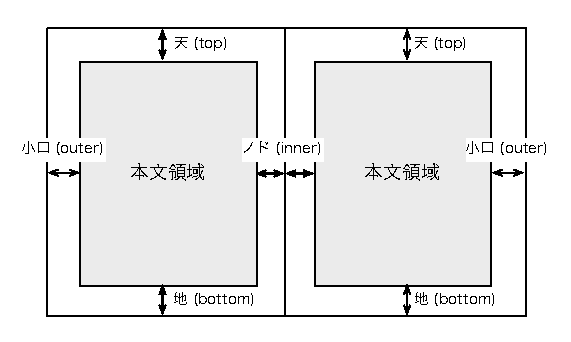
\includegraphics{name}
  \caption{片面印刷時の用紙各部の名称}
 \end{center}
\end{figure}

\begin{figure}[htbp]
 \begin{center}
  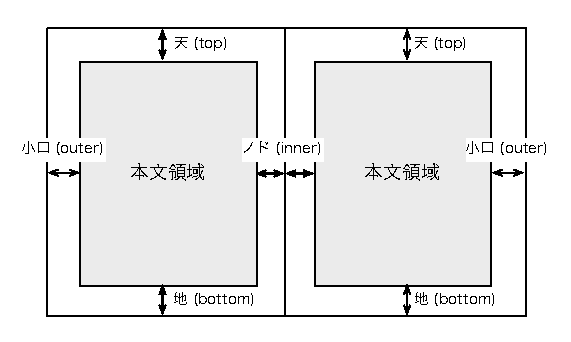
\includegraphics{name}
  \caption{両面印刷時の用紙各部の名称}
 \end{center}
\end{figure}


%オプションについては後述しますが,本書も\sty{geometry}パッケージを用いて,
%次のようにページ設定されています.

%\begin{intext}
%\usepackage[%showframe,% for debug
%  paperwidth=128mm,paperheight=182mm,% JIS B6
%  outer=15mm,inner=15mm,% 小口 = outer, ノド = inner
%  tmargin=16mm,bmargin=15mm,% 天 = tmargin, 地 = bmargin
%  headsep=.5\cvs,% 柱と本文の空き
%  ignorefoot,ignoremp]{geometry}% フッター・傍注は無視
%\end{intext}

\subsection{デバイスドライバを指定する}

\begin{description}
 \item[\Option{dvips}] \Prog{dvips}用に用紙サイズ情報を設定します.
 \item[\Option{dvipdfm}] \Prog[dvipdfm]{\Dvipdfm}用に用紙サイズ情報を設
 定します.
 \item[\Option{pdftex}] \Prog[pdftex]{\PDFTeX},
 \Prog[pdflatex]{\PDFLaTeX}用に用紙サイズ情報を設定します.
\end{description}

\subsection{デバッグ情報を表示する}
\begin{description}
 \item[\Option{verbose}] 
  \Y{geometry}パッケージの処理内容を詳細に表示します.
 \item[\Option{showframe}] 
  ページレイアウトの設定を確認するために,1ページ目の本文領域,ヘッダー,
  フッターを枠で囲みます.
\end{description}


\subsection{用紙サイズを指定する}
\begin{usage}
\geometry{$\<既定のサイズ>$}
\geometry{papersize=$\<用紙の幅>$,$\<用紙の高さ>$}
\geometry{paperwidth=$\<用紙の幅>$}
\geometry{paperheight=$\<用紙の高さ>$}
\end{usage}

\val{既定のサイズ}には以下のオプションがあります.
\begin{description}
 \item[既定のサイズ]
\zindind{用紙}{の既定のサイズ}
  \Optionlist{a0paper,a1paper,a2paper,a3paper,a4paper,a5paper,a6paper,%
  b0paper,b1paper,b2paper,b3paper,b4paper,b5paper,b6paper,%
  letterpaper,executivepaper,legalpaper,screen}.
  \option{screen} は 225\,mm $\times$ 180\,mm になります.
  \option{screen}は\option{centering} も併用すると便利です.
  `\str{paper=}\val{用紙サイズ}'と記述しても大丈夫です.
    ただし,B列の用紙はJISではなくISOのサイズであるため,JISのB5にしたけ
    れば,直接以下の\option{papersize}オプションを使って
    \verb|papersize={182mm,257mm}| とする必要があります.
\item[\Option{paperwidth}] 
\zindind{用紙}{の幅}
  \Z{用紙}の幅を,\val{長さ}を指定して決めます.
  `\str{paperwidth=10cm}'のように使います.
\item[\Option{paperheight}]
\zindind{用紙}{の高さ}
  用紙の高さを,\val{長さ}を指定して決めます.
\item[\Option{papersize}]
  `\option{papersize}\str=\twoargs{幅}{高さ}'とするか,
  `\option{papersize}\str=\val{長さ}'とすれば \option{paperwidth}
  と\option{paperheight}を用いた事と等価になります.
\end{description}

%JIS~B6にする.
%\begin{intext}
%\usepackage[paperwidth=128mm,paperheight=182mm]{geometry}
%\end{intext}

\subsection{用紙の方向を指定する}
\begin{description}
\item[\Option{landscape}] 
  \Z{横置き}でページレイアウトを設定します.
\item[\Option{portrait}]
  \Z{縦置き}でページレイアウトを設定します.
\end{description}


\subsection{紙面で本文領域が占める割合を指定する}

\begin{description}
 \item[\Option{hscale}] 
  用紙の幅 (\C{paperwidth}) に対して本文領域が占める横幅の比率です.
  `\str{hscale=.8}' とすると `\str{width=.8\BS paperwidth}' と等価になりま
  す.標準は 0.7 です.
 \item[\Option{vscale}] 
  用紙の高さ (\C{paperheight}) に対して本文領域が占める高さの比率です.
  `\str{vscale=.8}' とすると `\str{height=.9\BS paperheight}' と等価になりま
  す.標準は 0.7 です.
 \item[\Option{scale}] 
  本文が幅と高さに関して用紙に対して占める比率を指定します.
  `\str{scale=}\twoargs{幅の比率}{高さの比率}'
   とするか`\str{scale=}\val{比率}'として使います.標準は 0.7 です.
\end{description}

\subsection{本文領域の幅・高さの長さを直接指定する}
\begin{description}
 \item[\Option{width}/\Option{totalwidth}] 
\indindz{幅}{本文のトータルな}
  本文のトータルな幅を指定します.`\str{width=}\val{長さ}'とするか,
  `\str{totalwidth=}\val{長さ}'とします.
 \item[\Option{height}/\Option{totalheight}] 
\indindz{高さ}{本文のトータルな}
  本文のトータルな高さを指定します.`\str{height=}\val{長さ}'とするか,
  `\str{totalheight=}\val{長さ}'とします.
 \item[\Option{total}] 
  本文のトータルな幅と高さを指定します.
  `\str{total=}\twoargs{幅}{高さ}'とするか,
  `\str{total=}\val{長さ}'とします.
 \item[\Option{textwidth}] 
   文章領域となる \C{textwidth} の幅を指定します.
   `\str{textwidth=}\val{長さ}'とします.
 \item[\Option{textheight}]
   文章領域となる \C{textheight} の高さを指定します.
   `\str{textheight=}\val{長さ}'とします.
 \item[\Option{text}/\Option{body}]
  \C{textwidth} と \C{textheight} の両方を指定します.
  `\str{body=}\twoargs{幅}{高さ}'とするか`\str{text=}\val{長さ}'とします.
\end{description}



\subsection{1行の文字数を指定する}
\begin{usage}
\geometry{textwidth=$\<文字数>$zw}
\end{usage}

\subsection{本文の高さを行送りの倍数にする}

%\begin{usage}
%\setlength{\baselineskip}{$\<行の高さ>$} 
%\end{usage}

\begin{description}
  \item[\Option{heightrounded}]
  本文の高さが行送りの倍数でない場合に,``\str{underfull vbox}''の警告を
  出さないように \C{textheight} を \val{\C{baselineskip} の整数倍 $+$
  \C{topskip}} にします.
\end{description}

\subsection{1ページの行数を指定して本文の高さを決める}
%\begin{usage}
%\setlength{\textheight}{$\<行数>$\baselineskip} 
%\end{usage}
%しかし,
%\begin{intext}
%\advance\textheight\topskip
%\end{intext}
%しないと適切に処理されない.

\begin{usage}
\usepackage{geometry}
\geometry{lines=$\<行数>$} 
\end{usage}

\begin{description}
 \item[\Option{lines}]
  \cmd{textheight} を\Z{行数}によって決めます.`\str{lines=}\val{整数}'で指定
  します.
\end{description}

\subsection{ヘッダ・フッタ領域を本文の高さに含める/含めない}

\begin{description}
 \item[\Option{includehead}]
  トータルな本文の高さ\option{height}/\option{totalheight}にヘッダー
  (\C{headheight} と \C{headsep}) を含めるようにします.標準では無効です.
 \item[\Option{includefoot}]
  トータルな本文の高さ\option{height}/\option{totalheight}にフッター
  (\C{footskip}) を含めるようにします.標準では無効です.
 \item[\Option{includeheadfoot}]
  \option{includehead} と \option{includefoot} の両方を有効にします.
\end{description}

\begin{description}
 \item[\Option{ignorehead}]
  トータルな本文の高さにヘッダーを含めないようにします.標準で有効です.
  `\str{includehead=false}'とするのと等価です.
 \item[\Option{ignorefoot}]
  トータルな本文の高さにフッターを含めないようにします.標準で有効です.
  `\str{includefoot=false}'とするのと等価です.
 \item[\Option{ignoreheadfoot}]
  \option{ignorehead} と \option{ignorefoot} の両方を指定した事と等価で
  す.
\end{description}

\subsection{傍注領域を本文の幅に含める/含めない}

\begin{description}
 \item[\Option{includemp}]
  トータルな本文の幅に\Z{傍注} (\C{marginparwidth} と \C{marginparsep}) も
  含めるようにします.\Option{marginparwidth}と\Option{marginparsep}オプ
  ションに依存しています.標準では無効です.
 \item[\Option{ignoremp}]
  トータルな本文の幅に傍注を含めないようにします.標準で有効です.
\end{description}

\subsection{ヘッダ・フッタ・傍注領域を本文領域に含める/含めない}

\begin{description}
  \item[\Option{includeall}]
  \option{includeheadfoot} と \option{includemp} の両方を指定した事と等
  価です.
 \item[\Option{ignoreall}]
  \option{ignoreheadfoot} と \option{ignoremp} の両方を指定した事と等価
  です.
\end{description}


\subsection{本文領域と余白の長さを直接指定する}

\begin{description}
 \item[\Option{hdivide}]
  左余白,文章の幅,右余白を指定します.`\str{hdivide=}%
  \threeargs{左余白}{文章幅}{右余白}'のように使います.
  このオプションは三つのうち二つだけ明確な時に,不定の一つを星`\str{*}'
  に置き換えて`\verb|hdivide={2cm,15cm,*}|'とできます.
 \item[\Option{vdivide}]
  \Z{上余白},文章の高さ,\Z{下余白}を指定します.`\str{vdivide=}%
  \threeargs{上余白}{文章幅}{下余白}'のように使います.
 \item[\Option{divide}]
  `\str{divide=}\threeargs{長さ\mbox{$_1$}}{長さ\mbox{$_2$}}{長さ
  \mbox{$_3$}}'とすると`\str{hdivide=}\threeargs{長さ\mbox{$_1$}}{長さ
  \mbox{$_2$}}{長さ\mbox{$_3$}}'と\str{vdivide=}\threeargs{長さ
  \mbox{$_1$}}{長さ\mbox{$_2$}}{長さ\mbox{$_3$}}'を指定した事と等価にな
  ります.
\end{description}


\subsection{余白の長さ指定する}

\begin{description}
 \item[\Option{left}/\Option{lmargin}/\Option{inner}]
 \zindind{用紙}{の左端}
 用紙の左端と本文領域(版面)とのあいだにある左余白を指定します.
 `\str{lmargin=}\val{長さ}'のように使います.両面印刷指定
 (\Option{twoside}) の場合は\Z{ノド}の長さを設定します.
 \item[\Option{right}/\Option{rmargin}/\Option{outer}]
 \zindind{用紙}{の右端}
 用紙の右端と本文領域とのあいだにある右余白を指定します.
 `\str{rmargin=}\val{長さ}'のように使います.両面印刷指定
 (\Option{twoside}) の場合は\Z{小口}の長さを設定します.
 \item[\Option{top}/\Option{tmargin}]
  用紙の上端と本文領域のとのあいだ(\Z{天})にある上余白を指定します.
 `\str{tmargin=}\val{長さ}'のように使います.
 \item[\Option{bottom}/\Option{bmargin}]
  用紙の下端と本文領域のとのあいだ(\Z{地})にある下余白を指定します.
 `\str{bmargin=}\val{長さ}'のように使います.
 \item[\Option{hmargin}]
  左右余白を指定します.`\str{hmargin=}\twoargs{左余白}{右余白}'とするか,
  `\str{hmargin=}\val{長さ}'とします.
 \item[\Option{vmargin}]
  上下余白を指定します.`\str{vmargin=}\twoargs{上余白}{下余白}'とするか,
  `\str{vmargin=}\val{長さ}'とします.
 \item[\Option{margin}]
  `\str{margin=}\twoargs{長さ\mbox{$_1$}}{長さ\mbox{$_2$}}'とすると,
  `\str{hmargin=}\twoargs{長さ\mbox{$_1$}}{長さ\mbox{$_2$}}'と
  `\str{vmargin=}\twoargs{長さ\mbox{$_1$}}{長さ\mbox{$_2$}}'を指定した
  事と等価になります.
\end{description}

\subsection{余白の比率を指定する}

\begin{description}
 \item[\Option{hmarginratio}]
  左右余白の比率を指定します.`\str{hmarginration=}\val{左の比率\str:右の比率}'
  のようにコロンで区切ります.正の整数値で 100 以下である必要があります.
  片面印刷時 (\Option{oneside}) は $1:1$, 両面印刷時 (\Option{twoside})
  は $2:3$ が標準です.
  \item[\Option{vmarginratio}]
  用紙の上余白と下余白(\Z{天地})の比率を指定します.
 \item[\Option{marginratio}]
  `\str{marginratio=}\twoargs{左右の比率}{上下の比率}'とするか,
  `\str{marginration=}\val{比率}'とします.
 \item[\Option{hcentering}]
  `\str{hmarginratio=1:1}'とした事と等価になります.
 \item[\Option{vcentering}]
  `\str{vmarginratio=1:1}'とした事と等価になります.
 \item[\Option{centering}]
  `\str{marginratio=1:1}'とした事と等価になります.
\end{description}

\subsection{両面印刷用に余白を調整する}

\begin{description}
 \item[\Option{twoside}]
 \zindind{左右}{対称}
  \Z{両面印刷}時に文章領域(\Z{版面})が左右対称になるようにします.
 \item[\Option{twoside}] 
HOGEHOGE
  両面印刷用に傍注の位置を入れ換え,紙面を左右対称になるようにします.
HOGEHOGE
 \item[\Option{asymmetric}]
 \zindind{左右}{非対称}
  両面印刷時に文章領域が左右非対称になるようにします.ただし,
  \option{bindingoffset}は考慮されます.
 \item[\Option{bindingoffset}]
  \zindind{文書}{を綴じる}
  \Z{片面印刷}時でも両面印刷時においても文書を綴じる背の部分の余白を
  指定します.`\str{bindingoffset=}\val{長さ}'として使います.
\end{description}

\subsection{ヘッダの高さ・フッタと本文の空きを指定する}
\begin{description}
 \item[\Option{headheight}/\Option{head}] 
  `\str{head=}\val{長さ}'として \C{headheight} を設定します.
 \item[\Option{headsep}] 
  `\str{headsep=}\val{長さ}'として \C{headsep} を設定します.
 \item[\Option{footskip}/\Option{foot}] 
  `\str{foot=}\val{長さ}'として \C{footskip} を設定します.
\end{description}


\subsection{ヘッダ・フッタを無しに設定する}
\begin{description}
 \item[\Option{nohead}] 
  ヘッダー無しの設定にします(\C{headheight} と \C{headsep} を 0\,pt
  にします).
 \item[\Option{nofoot}] 
  フッター無しの設定にします(\C{footskip} を 0\,ptにします).
 \item[\Option{noheadfoot}] 
  \option{nohead} と \option{nofoot} を指定した事と等価になります.
\end{description}

\subsection{傍注の幅・本文との空きなどを指定する}
\begin{description}
 \item[\Option{marginparwidth}/\Option{marginpar}] 
 \zindind{傍注}{の幅}
  `\str{marginpar=}\val{長さ}'として傍注の幅 \C{marginparwidth} を設定し
  ます.
 \item[\Option{marginparsep}]
 \zindind{傍注}{と本文の空き}
  `\str{marginparsep=}\val{長さ}'として傍注と本文の空き \C{marginparsep}
  を設定します. 
 \item[\Option{nomarginpar}]
  傍注無しの設定にします(\C{marginparwidth} と \C{marginparsep} を
  0\,pt にします).
 \item[\Option{reversemp}/\Option{reversemarginpar}]
 傍注の位置を非標準の左側に出力するようにします.両面印刷時は
 \Z{見開き}の内側(小口)に設定します.
\end{description}

\subsection{オフセットを調整する}
\begin{description}
 \item[\Option{hoffset}]
  `\str{hoffset=}\val{長さ}'として \C{hoffset} を設定します.
 \item[\Option{voffset}]
  `\str{voffset=}\val{長さ}'として \C{voffset} を設定します.
 \item[\Option{offset}]
  `\str{offset=}\twoargs{水平方向のオフセット量}{垂直方向のオフセット量}'と
  するか`\str{offset=}\val{オフセット量}'として,\Z{オフセット}を指定します.
\end{description}

\subsection{2段組みに設定する}

\begin{description}
 \item[\Option{columnsep}]
  `\str{columnsep=}\val{長さ}'として\Z{段間}の空き \C{columnsep} を設定します.
 \item[\Option{twocolumn}]
  2段組の設定にします.
\end{description}

\subsection{具体的な設定例を見る}

\makeatletter
\newcommand*\geoimage[2][clip]{%
  \noindent
  \hbox{\includegraphics[scale=1,#1]{geolay/geo#2-2-crop.pdf}}%
  \nobreakspace
  \hbox{\includegraphics[scale=1,#1]{geolay/geo#2-1-crop.pdf}}%
}
\newcommand*\GQ{,}
\newcommand\geooptionlist[1]{
 \@for\member:=#1\do{\advance\@tempcnta\@ne}%
 \@for\member:=#1\do{\advance\@tempcntb\@ne
   \ifnum\@tempcntb<\@tempcnta
         \texttt{\member},\\
 \else
  \ifnum\@tempcntb=\@tempcnta
    \texttt{\member}%
  \fi
\fi}%
}
%\newcommand*\GeoOptions[2][7em]{%\geooptionlist{#1}%
% \fbox{\parbox[b]{#1}{\geooptionlist{#2}}}%
%}
\newcommand\GEO[5][\geoimage]{%
\par\vskip.5\cvs
\noindent\makebox[0pt][l]{%
   {\begin{minipage}[c]{#4\fullwidth}%
      \small \geooptionlist{#2}%
   \end{minipage}}%
   \hfil
   {%
    \begin{minipage}{#5\fullwidth}%
     \null\hfill #1{#3}%
   \end{minipage}%
   }%
}\par\vskip.5\cvs
}

\makeatother

\Cls{jsbook}クラスでのレイアウト例を示します.まずパッケージを読み込まな
い状態でのレイアウトです.

\GEO{パッケージ無し}{1}{.2}{.8}

%\begin{Prob}
%上下左右の余白をちょうど 2\,cm に設定するにはどうすれば良いか
%考えてください.%少なくとも解は一つ以上あります.
%\GEO{margin=2cm}{2}{.2}{.8}
%この場合はヘッダー,フッター,傍注の領域が含まれない事も確認してください.
%\end{Prob}

次は上下の余白の比率を $1:1$,左右の余白の比率を $1:1$ に
指定した例です.

\GEO{centering}{3}{.2}{.8}

この場合もヘッダー,フッター,傍注の領域は含まれません.
次は見開きの内側の余白を 1\,cm足した例です.

\GEO{twoside,bindingoffset=1cm}{4}{.2}{.8}

%\begin{Prob}
左余白を 3\,cm,右余白を 2\,cm,\Z{行数}を40行送り分,上余白を
2.5\,cmとして,ヘッダーとフッターの領域をトータルな高さに含める
ような \Y{geometry} の設定を考えてください.いくつも解答はありますが,
例えば次のような設定の実行結果を吟味してください.

\begin{intext}
\geometry{left=3cm,right=2cm,lines=40,top=2.5cm,includeheadfoot}
\end{intext}
%\GEO{left=3cm,right=2cm,lines=40,top=2.5cm,includeheadfoot}{5}{.2}{.8}

また,これは次のようにしても同じである事を確認してください.

\begin{intext}
\geometry{hmargin={3cm,2cm},tmargin=2.5cm,lines=40,includeheadfoot}
\end{intext}
%\end{Prob}

%\GEO{hmargin=\lb3cm\GQ2cm\rb,tmargin=2.5cm,lines=40,includeheadfoot}{6}

次は本文の高さを 10\,inch,下余白を 2\,cm,残りは上余白にするような
設定です.

\GEO{vdivide=\\\lb*\GQ10in\GQ2cm\rb}{7}{.2}{.8}

これは次のようにしても同じ事になります.

\begin{intext}
\geometry{bottom=2cm,textheight=10in}
\end{intext}

%\GEO{bottom=2cm,textheight=10in,includefoot}{8}

次は幅も高さも用紙の 80\% だけ本文の領域に割り当てるようにし,
用紙の中央に本文が配置するようにします.

\GEO{scale=0.8,centering}{9}{.2}{.8}

用紙サイズを A5 とし,傍注の幅を 3\,cm,傍注の幅もトータルな幅に含めるよ
うにします.

\GEO{a5paper,marginparwidth=3cm,includemp}{10}{.3}{.7}

次は用紙サイズを B4 とし,横置き,2段組,左右上下の余白は2\,cm,
傍注・ヘッダー・フッターなしで,段間の幅を 2\,cm とします.

A4 以外の用紙サイズでは dvipdfm のように,デバイスドライバを指定した
方が良いかも

\GEO[\includegraphics]{dvipdfm,b4paper,landscape,twocolumn,margin=2cm,nomarginpar,nofoot,nohead,columnsep=2zw}{geolay/geo11-1-crop.pdf}{.2}{.8}
%\hbox{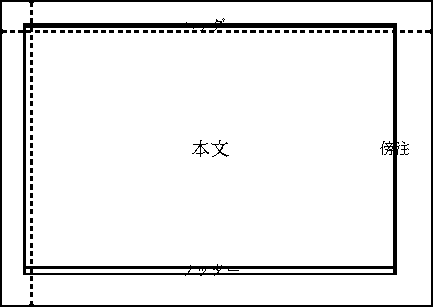
\includegraphics[scale=1]{geolay/geo11-1-crop.pdf}}%

%  vmargin=25mm,hmargin=15mm,
%  tmargin=25mm,bmargin=25mm,lmargin=15mm,rmargin=15mm,
%  top=25mm,bottom=25mm,left=15mm,right=15mm,

次は用紙サイズを A4 として,2段組,左右余白をそれぞれ 15\,mm,
上下余白を 25\,mm,段間の幅を 6\,mm,傍注・ヘッダー・フッター
なしの設定にします.

\GEO[\includegraphics]{a4paper,twocolumn,ignoreall,nomarginpar,noheadfoot,margin=\lb15mm\GQ25mm\rb,columnsep=6mm}{geolay/geo12-1-crop.pdf}{.3}{.7}
%\hbox{[scale=1]{geolay/geo12-1-crop.pdf}}%


\endinput
% geometry
\subsection{クラスファイルで提供されているスタイルを切り替える}
\begin{usage}
 \pagestyle{$\<スタイル>$}% 該当ページ以降を変更する
 \thispagestyle{$\<スタイル>$}% 該当ページのみを変更する
\end{usage}

\begin{description}
 \item[empty]  
 \item[plain] 
 \item[headings] 
 \item[myheadings] 
\end{description}

%\subsection{ヘッダやフッタの設定その1}\indindz{番号}{ページ}%
ヘッダやフッタなどに出力されるページ番号などを\zindind{ページ}{の番号}
変更したいときがあると思います.
\begin{usage}
\pagestyle{$\<表示形式>$}
\end{usage}

\C{pagestyle}命令を記述したページから指定した\Z{表示形式}に変更されま
す.指定できる形式は\tabref{pagestyle}の通りです.


\begin{table}[htbp]
\begin{center}
\caption{ヘッダやフッタの指定}\tablab{pagestyle}
\begin{tabular}{ll}
\TR
\Th{命令}        & \Th{内容} \\
\MR
\str{empty}      & ページ番号を表示しない                \\
\str{plain}      & フッタ中央部に表示する              \\
\str{headings}   & ヘッダにページ番号と章・節名を表示する\\
\str{myheadings} & ユーザ定義の表示形式にする          \\
\BR
\end{tabular}
\end{center}
\end{table}

\qu{\str{myheadings}}では二つの命令によってヘッダの出力を指定します.

\begin{usage}
\markright{$\<ヘッダ>$}
\markboth{$\<偶数ヘッダ>$}{$\<奇数ヘッダ>$}
\end{usage}


片面印刷のときに \cmd{markright}を使います.
両面印刷には \C{markboth}を使います.
2007年度版の「○○△△大学」の論文集を
作成しているのであれば,例えば次のようにします.

\begin{intext}
\pagestyle{myheadings}
\markboth{○○△△大学論文集}{2007年度版}
\end{intext}


任意の1ページだけのヘッダ・フッタは,
次のようにする事でそのページだけ変えられます.

\begin{usage}
\thispagestyle{$\<表示形式>$}
\end{usage}


ページ番号の表示形式を変更するには \C{pagenumbering}命令を使います.

\begin{usage}
\pagenumbering{$\<表示形式>$}
\end{usage}

その場所から指定した形式で1ページ目からカウントしてページ番号を表示しま
す.指定できる表示形式は\tabref{pagenumber}の通りです.

\begin{table}[htbp]
\begin{center}
\caption{ページ番号の種類の指定}\tablab{pagenumber}
\begin{tabular}{lll}
\TR
\Th{形式}          & \Th{内容}          & \Th{出力例}         \\
\MR
\verb+arabic+ & \Z{アラビア数字}       & 1, 2, 3,\,\ldots \\
\verb+roan+   & 小文字の\Z{ローマ数字}   & i, ii, iii,\,\ldots\\
\verb+Roman+  & 大文字のローマ数字   & I, II, III,\,\ldots\\
\verb+alph+   & アルファベット小文字& a, b, c,\,\ldots,\, z\\
\verb+Alph+   & アルファベット大文字& A, B, C,\,\ldots,\, Z\\
\BR
\end{tabular}
\end{center}
\end{table}
ここで注意する事はアルファベットにした場合は,
最大26ページまでしかカウントできないという事
です.27以上になった場合の対策は別にする事に
なります.

%もっと詳細なヘッダ・フッタ定義するときは自分で
%\cmd{ps@なんとか}というコマンドを定義してこれを
%\begin{intext}
%pagestyle{なんとか} 
%\end{intext}
%のように使います.本書で使われているスタイルは
%以下の通りです.\hito{奥村}{晴彦}の\cls{jsclasses}
%を少し変更しただけです.
%\begin{intext}
%\newcommand{\ps@myhead}{%
%  \let\@oddfoot\@empty
%  \let\@evenfoot\@empty
%  \def\@evenhead{%
%    \if@mparswitch \hss \fi
%    \underline{\hbox to \fullwidth{\autoxspacing
%        \textbf{\thepage}\hskip3zw\leftmark\hfill\@title}}%
%    \if@mparswitch\else \hss \fi}%
%  \def\@oddhead{\underline{\hbox to \fullwidth{\autoxspacing
%        \@title\hfill{\if@twoside\rightmark\else\leftmark\fi}%
%	\hskip3zw\textbf{\thepage}}}\hss}%
%  \let\@mkboth\markboth
%  \def\chaptermark##1{\markboth{%
%    \ifnum \c@secnumdepth >\m@ne
%      \if@mainmatter
%        \@chapapp\thechapter\@chappos\hskip1zw
%      \fi
%    \fi
%    ##1}{}}%
%  \def\sectionmark##1{\markright{%
%    \ifnum \c@secnumdepth >\z@ \thesection \hskip1zw\fi
%    ##1}}}%
%\end{intext}
%これを別ファイル\fl{hoge.sty}などにまとめて\cmd{usepackage}
%するか,\cmd{makeatletter}と\cmd{makeatother}で囲むかで
%実際の出力を確認してみてください.
% LaTeX 標準ヘッダ・フッタ設定
\section{\Y{fancyhdr}によるヘッダ・フッタの設定}

%\section{ヘッダ・フッタの変更その2\zdash\Y{fancyhdr}}
\indindz{スタイル}{ページ}%
\zindind{ページ}{スタイル}%
{\LaTeX}が標準で用意してくれているページスタイル
では寂しい,そう思う人も多いでしょう.自分で全て
定義する事もできますが,\Person{Piet}{Oostrum}が
作成した \Y{fancyhdr} を使うと比較的簡単にペー
ジスタイルをカスタマイズできます.\sty{fancyhdr}
は\Y{fancyheadings}の後継で,ページのヘッダーと
フッターをカスタマイズできるマクロです.
まず\sty{fancyhdr}を使うために以下をプリアンブルに記述します.

\begin{intext}
\usepackage{fancyhdr} 
\pagestyle{fancy}
\end{intext}

\sty{fancyhdr}では
ヘッダ・フッタを六つに分割しています.
\begin{center}
\begin{tabularx}{.8\linewidth}{|XcX|}
\hline
\cmd{lhead} & \cmd{chead} & \hfill\cmd{rhead}\\
\multicolumn{3}{|c|}{%
   \hrulefill (\C{headrulewidth})\hrulefill} \\   
\multicolumn{3}{|c|}{\val{本文領域}}\\
\multicolumn{3}{|c|}{%
   \hrulefill (\C{footrulewidth})\hrulefill} \\
\cmd{lfoot} & \cmd{cfoot} &\hfill\cmd{rfoot} \\
\hline
\end{tabularx}
\end{center}
\C{lhead},\C{chead},\C{rhead}の
三つはヘッダに使い\C{lfoot},\C{cfoot},
\C{rfoot}の三つはフッタに使います.%
\indindz{罫線}{ヘッダ上部の}\indindz{罫線}{フッタ上部の}%%
\C{headrulewidth}はヘッダ下部の罫線の太さで,
\C{footrulewidth}はフッタ上部の罫線の太さです.
図だけのページや表だけのページはシンプルな
ヘッダ・フッタにしたり,ヘッダ下部の罫線を
引かない場合があります.その場合は \C{headrulewidth} を
\C{iffloatpage}命令で判定するように定義すると良いでしょう.

\begin{intext}
\def\headrulewidth{\iffloatpage{0pt}{.4pt}} 
\end{intext}

\cmd{lhead}などの
他の命令も同様に変更できます.

例えば\cls{jarticle}クラスで次のようなヘッダ・フッタ
\begin{center}
\begin{tabularx}{\linewidth}{|cXcXc|}
\hline
& & \hskip5em & \hfill 資本主義社会の崩壊 & \\
\cline{2-4}
\multicolumn{5}{|c|}{\val{本文領域}}\\
\cline{2-4}
& 名無しの権兵衛 & \hskip3em & \hfill \textbf{ページ番号} & \\
\hline
\end{tabularx}
\end{center}
を設定したければ以下のように記述します.

\begin{intext}
\lhead{} \chead{}
\rhead{資本主義社会の崩壊}
\lfoot{名無しの権兵衛} 
\cfoot{}
\rfoot{\textbf{\thepage}}
\def\headrulewidth{.4pt}
\def\footrulewidth{.4pt}
\end{intext}

書籍用クラス\cls{jbook}などでクラスオプションに
\Option{twoside}が指定されている場合は偶数ページと
奇数ページを個々に設定します.例えば次のような
ヘッダ・フッタにしたいとします.
\begin{center}
\begin{tabular}{|p{7zw}cp{7zw}|}
\hline
第1章\hskip1zw 序論& & \hfill 1.1\hskip1zw 背景\\\hline
\multicolumn{3}{|c|}{本文}\\\hline
& \textbf{2}&\hfill \\\hline
\end{tabular} \hfill
\begin{tabular}{|p{7zw}cp{7zw}|}
\hline
1.2\hskip1zw  目標& & \hfill 第1章\hskip1zw 序論\\\hline
\multicolumn{3}{|c|}{本文}\\\hline
& \textbf{3}& \\\hline
\end{tabular}
\end{center}
ヘッダ・フッタの奇数ページと偶数ページの場所
を区別するために以下のような設定になっています.
\begin{center}
\begin{tabular}{|p{6zw}cp{6zw}|}
\hline
\str{EL(H)}& \str{EC(H)}& \hfill  \str{ER(H)}\\\hline
\multicolumn{3}{|c|}{本文}\\\hline
\str{EL(F)}& \str{EC(F)} &\hfill \str{ER(F)} \\\hline
\multicolumn{3}{c}{偶数ページ側}\\
\end{tabular} \hfill
\begin{tabular}{|p{6zw}cp{6zw}|}
\hline
\str{OL(H)} &\str{OC(H)} & \hfill \str{OR(H)} \\\hline
\multicolumn{3}{|c|}{本文}\\\hline
\str{OL(F)}&\str{OC(F)} & \hfill  \str{OR(F)}\\\hline
\multicolumn{3}{c}{奇数ページ側}\\
\end{tabular}
\end{center}
先程の出力を得るためには \C{fancyhead} と \C{fancyfoot}命令を使います.

\begin{intext}
\documentclass{jbook}
\usepackage{fancyhdr} \pagestyle{fancy}
\fancyhead[ER,OL]{\rightmark}
\fancyhead[EL,OR]{\leftmark}
\fancyfoot[EC,OC]{\textbf{\thepage}}
\end{intext}

欧文のクラスではこれで良いのですが和文では \C{chaptermark} 
と \C{sectionmark}の定義を\sty{fancyhdr}を読み込んだ後に次のように定義
するのが良いでしょう.

\begin{intext}
 \def\chaptermark#1{\markboth{%
   \ifnum \c@secnumdepth >\m@ne
     \if@mainmatter
       \@chapapp\thechapter\@chappos\hskip1zw
     \fi
   \fi
   #1}{}}%
  \def\sectionmark#1{\markright{%
    \ifnum \c@secnumdepth >\z@ \thesection \hskip1zw\fi
    #1}}%
\end{intext}

\subsection{標準設定}
\begin{intext}
\usepackage{fancyhdr} 
\usepackage{fancy}
\fancyhead[LE,RO]{\slshape \rightmark}
\fancyfoot[LE,RE]{\slshape \leftmark}
\renewcommand*{\headrulewidth}{0.4pt}
\renewcommand*{\footrulewidth}{0.4pt}
\end{intext}

標準では見出しが uppercase に変更される.

\begin{usage}
\lhead{\nouppercase{\rightmark}} 
\rhead{\nouppercase{\leftmark}}
\end{usage}

\subsection{chaptermark, sectionmark 再定義}

\begin{intext}
\renewcommand{\chaptermark}[1]{%
   \markboth{\chaptername\ \thechapter.\ #1}{}}
\end{intext}

\subsection{片面印刷時のヘッダ・フッタ設定}

\CIS{lhead,chead,rhead,lfoot,cfoot,rfoot,headrulewidth,footrulewidth}%
\begin{usage}
\lhead{$\<ヘッダ左側>$}
\chead{$\<ヘッダ中央>$}
\rhead{$\<ヘッダ右側>$}
\lfoot{$\<フッタ左側>$}
\cfoot{$\<フッタ中央>$}
\rfoot{$\<フッタ右側>$}
\end{usage}

\subsection{両面印刷時のヘッダ・フッタ設定}
\begin{usage}
\fancyhead{} % to clear all fields
\fancyhead[$\<位置指定>$]{$\<ヘッダ要素>$}
\fancyfoot[$\<位置指定>$]{$\<フッタ要素>$}
\end{usage}

\subsection{罫線}
\begin{usage}
\renewcommand*{\headrulewidth}{$\<ヘッダ下部の罫線の太さ>$}
\renewcommand*{\footrulewidth}{$\<フッタ上部の罫線の太さ>$}
\end{usage}

\subsection{ページ下部中央に「---\protect\val{ページ番号}---」だけ出力する}

\begin{usage}
\fancypagestyle{plain} 
\fancyhf{}
\fancyfoot[c]{---\bfseries\thepage---}
\renewcommand{\headrulewidth}{0pt}
\renewcommand{\footrulewidth}{0pt}
\end{usage}

\subsection{ヘッダ・フッタを2行にする}

\begin{intext}
\addtolength{\headheight}{\baseilneskip}
\renewcommand{\sectionmark}{\markboth{#1}{}}
\renewcommand{\subsectionmark}{\markright{#1}}
\rhead{\leftmark\\ \rightmark}
\end{intext}


\subsection{総ページ数を追加する}

ヘッダ・フッタの設定をフッタだけに「ページ/総ページ」にしたい場合がある
でしょう.これは例えば次のようにプリアンブルに記述します.

\begin{usage}
\usepackage{lastpage}
\cfoot{\thepage/\pageref{LastPage}}
\end{usage}

%この場合は \cmd{ps@total}によって新規に\qu{\str{total}}という
%ページスタイルを定義しています.ページ番号の書体を
%変えたいときは \cmd{normalfont}を \cmd{bfseries}などに
%変更します.

% fancyhdr
\section{段落・数式・浮動体のレイアウトパラメータ}

\subsection{段落レイアウト}

\begin{figure}[htbp]
 \begin{center}
  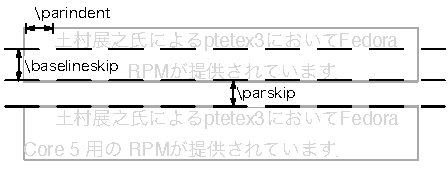
\includegraphics{layout-paragraph}
  \caption{段落設定のパラメータ}\figlab{段落設定のパラメータ}
 \end{center}
\end{figure}

\subsection{インデントを設定する}

\subsection{段落同士の空きを調整する}



\subsection{数式レイアウト}

\begin{figure}[htbp]
 \begin{center}
  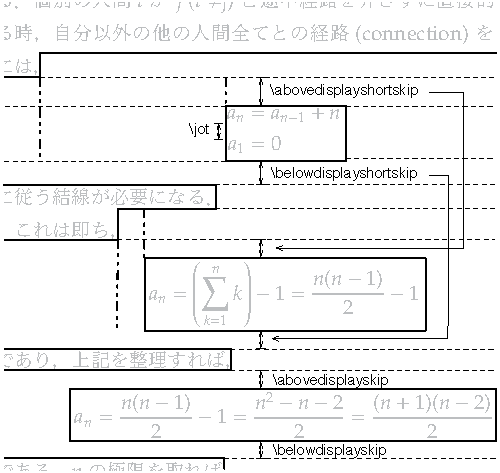
\includegraphics{layout-math}
  \caption{数式レイアウトのパラメータ}\figlab{数式レイアウトのパラメータ}
 \end{center}
\end{figure}

\subsection{fleqn}

\begin{figure}[htbp]
 \begin{center}
  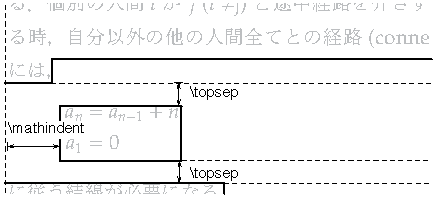
\includegraphics{layout-math-fleqn}
  \caption{fleqn数式レイアウトのパラメータ}\figlab{fleqn数式レイアウトのパラメータ}
 \end{center}
\end{figure}

\subsection{浮動体配置のパラメータ}

\begin{figure}[htbp]
 \begin{center}
  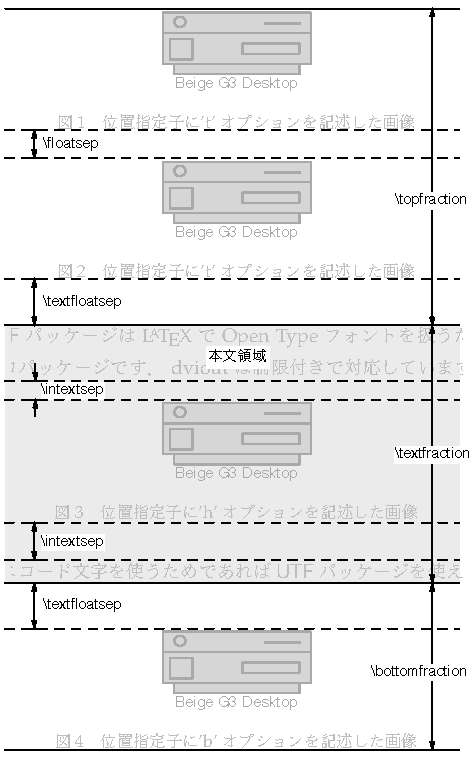
\includegraphics{layout-float}
  \caption{浮動体配置のパラメータ}\figlab{浮動体配置のパラメータ}
 \end{center}
\end{figure}


\C{dbltopnumber}
\C{dbltopfraction}
\C{dblfloatpagefraction}
\C{dblfloatsep}
\C{dbltextfloatsep}


\subsection{浮動体だけのページの書式パラメータ}

\C{floatpagefraction}
表が占めるべき最低の割合.% 段落・数式・フロート・レイアウト・パラメータ


